%%%%%%%%%%%%%%%%%%%%%%%%%%%%%%%%%%%%%%%%%
% Beamer Presentation
% LaTeX Template
% Version 1.0 (10/11/12)
%
% This template has been downloaded from:
% http://www.LaTeXTemplates.com
%
% License:
% CC BY-NC-SA 3.0 (http://creativecommons.org/licenses/by-nc-sa/3.0/)
%
%%%%%%%%%%%%%%%%%%%%%%%%%%%%%%%%%%%%%%%%%

%----------------------------------------------------------------------------------------
%	PACKAGES AND THEMES
%----------------------------------------------------------------------------------------

\documentclass[9pt]{beamer}
\usepackage{CJK}
\usepackage{ctex}
\usepackage{graphicx}
\usepackage{subfigure}
\usepackage{longtable}
\usepackage{rotating}
\usepackage{multirow}
\usepackage{algorithm}
\usepackage{algorithmic}
\usepackage{mathtools}
\usepackage{animate}
%\usepackage{media9}
%% A LATEX package for embedding interactive Adobe Flash (SWF) and 3D files (Adobe U3D & PRC) as well as video and sound files or streams (FLV, MP4/H.246, MP3) into PDF documents with Adobe Reader-9/X
%compatibility.
\renewcommand{\algorithmicrequire}{\textbf{Input:}}   %Use Input in the format of Algorithm
\renewcommand{\algorithmicensure}{\textbf{Output:}}  %UseOutput in the format of Algorithm
\newcommand{\e}[1]{\ensuremath{\times 10^{#1}}}
%\mode<presentation>{\usetheme{Madrid}}

\mode<presentation> {

% The Beamer class comes with a number of default slide themes
% which change the colors and layouts of slides. Below this is a list
% of all the themes, uncomment each in turn to see what they look like.

%\usetheme{default}
%\usetheme{AnnArbor}
%\usetheme{Antibes}
%\usetheme{Bergen}
%\usetheme{Berkeley}
%\usetheme{Berlin}
%\usetheme{Boadilla}
%\usetheme{CambridgeUS}
%\usetheme{Copenhagen}
%\usetheme{Darmstadt}
%\usetheme{Dresden}
%\usetheme{Frankfurt}
%\usetheme{Goettingen}
%\usetheme{Hannover}
%\usetheme{Ilmenau}
%\usetheme{JuanLesPins}
%\usetheme{Luebeck}
\usetheme{Madrid}
%\usetheme{Malmoe}
%\usetheme{Marburg}
%\usetheme{Montpellier}
%\usetheme{PaloAlto}
%\usetheme{Pittsburgh}
%\usetheme{Rochester}
%\usetheme{Singapore}
%\usetheme{Szeged}
%\usetheme{Warsaw}

% As well as themes, the Beamer class has a number of color themes
% for any slide theme. Uncomment each of these in turn to see how it
% changes the colors of your current slide theme.

%\usecolortheme{albatross}
\usecolortheme{beaver}
%\usecolortheme{beetle}
%\usecolortheme{crane}
%\usecolortheme{dolphin}
%\usecolortheme{dove}
%\usecolortheme{fly}
%\usecolortheme{lily}
%\usecolortheme{orchid}
%\usecolortheme{rose}
%\usecolortheme{seagull}
%\usecolortheme{seahorse}
%\usecolortheme{whale}
%\usecolortheme{wolverine}

%\setbeamertemplate{footline} % To remove the footer line in all slides uncomment this line
%\setbeamertemplate{footline}[page number] % To replace the footer line in all slides with a simple slide count uncomment this line

%\setbeamertemplate{navigation symbols}{} % To remove the navigation symbols from the bottom of all slides uncomment this line
}

\usepackage{graphicx} % Allows including images
\usepackage{booktabs} % Allows the use of \toprule, \midrule and \bottomrule in tables
\begin{document}
\begin{CJK*}{GBK}{kai}
%----------------------------------------------------------------------------------------
%	TITLE PAGE
%----------------------------------------------------------------------------------------

\title[Machine Learning]{Logistic Regression} % The short title appears at the bottom of every slide, the full title is only on the title page

%\author{Fuhao Zou(�޸���)}
\author{Fuhao Zou(�޸���)} % Your name
%\logo{%
%   
\includegraphics[scale=.2]{logo.pdf}\hspace*{4.75cm}~%
%   
\includegraphics[scale=.2]{logo.jpg}\hspace*{0.75cm}%
%   }
%\pgfdeclareimage[width=1cm]{hust}{logo.pdf}
%\logo{\pgfuseimage{hust}{\vspace{-10pt}}}
\titlegraphic{
\includegraphics[width=1.3cm]{logo.pdf}}
\institute[IEC, HUST] % Your institution as it will appear on the bottom of every slide, may be shorthand to save space
{
Intelligent and Embedded Computing Lab��\\
                   Huazhong University of Science \& Technology \\ % Your institution for the title page
\medskip
\textit{fuhao\_zou@hust.edu.cn} % Your email address
}

\date{2019��04��14��} % Date, can be changed to a custom date
%====================================================
\frame{\titlepage}

\frame{\frametitle{Table of contents}\tableofcontents}

\AtBeginSection[]
{
\begin{frame}{Table of Contents}
\tableofcontents[currentsection]
\end{frame}
}

%------------------------------------------------
%------------------------------------------------
\section{Linear Regression}
%------------------------------------------------
\subsection{Intorduction}
\begin{frame}
\frametitle{Intorduction}
\begin{block}{Basic idea:}
	\begin{itemize}
		\item function $$f(x)=\sum_{m=1}^{p}{w_mx_{im}+w_0}=w^Tx_i\eqno{(1)}$$
		\item $w_i$ are what the model learn through the samples
	\end{itemize}
\end{block}

\begin{figure}[h]
	\centering
	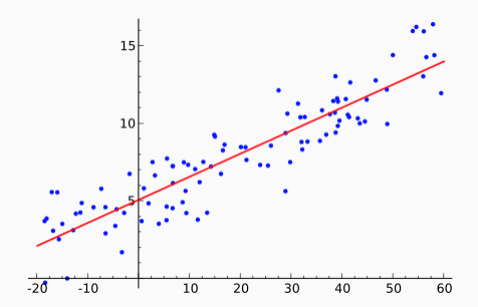
\includegraphics[scale=0.4]{1.png}
	\caption{Linear regression is a linear approach to modelling the relationship between input X and output Y.}
\end{figure}

\end{frame}
%------------------------------------------------
\subsection{Loss Function:}
\begin{frame}
\frametitle{Loss Function:}
\begin{block}{Basic idea}
\begin{itemize}
\item Loss function of Linear Regression-Least Square: $$
				J(w)=\frac{1}{n}\sum^n_{i=1}(y_i-f(x_i))^2=
				\frac{1}{n}||y-X_w||^2\eqno{(2)}
				$$
\item We seek the linear function of X that minimizes the sum of squared residuals from Y 
\end{itemize}
\end{block}
\begin{figure}[h]
	\centering
	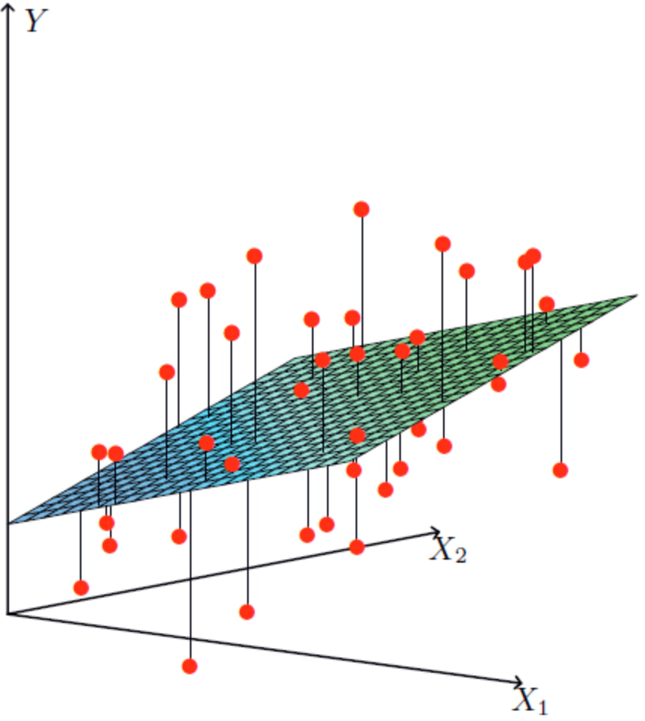
\includegraphics[scale=0.4]{2.png}
	
\end{figure}
\end{frame}

%------------------------------------------------
\subsection{Code Example}
\begin{frame}
\frametitle{Python Code}
\begin{figure}[h]
	\centering
	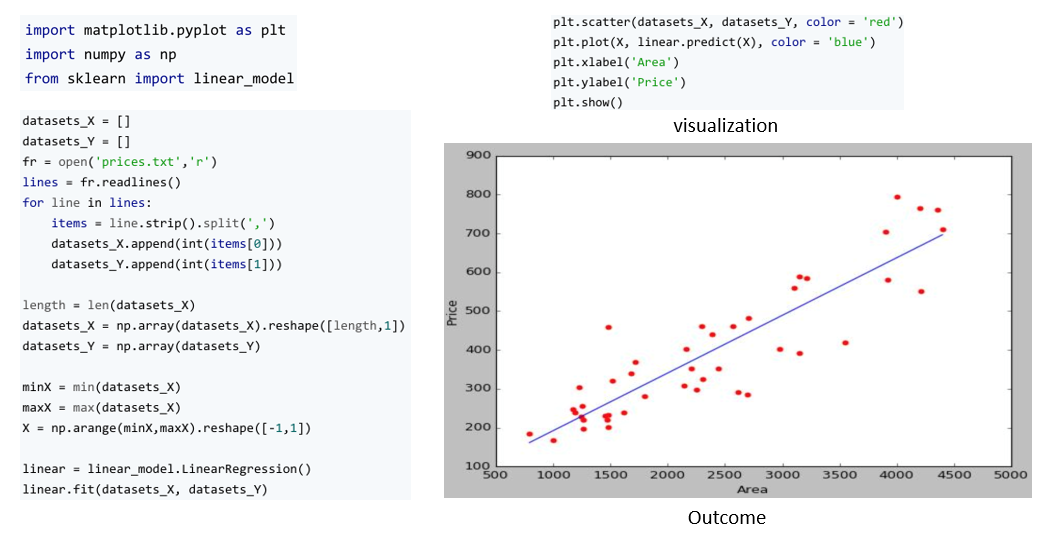
\includegraphics[scale=0.3]{3.png}
\end{figure}
\end{frame}
%------------------------------------------------

\section{Logistic Regression}
%------------------------------------------------
\subsection{Introduction}
\begin{frame}
\frametitle{Introduction}
\begin{figure}[h]
	\centering
	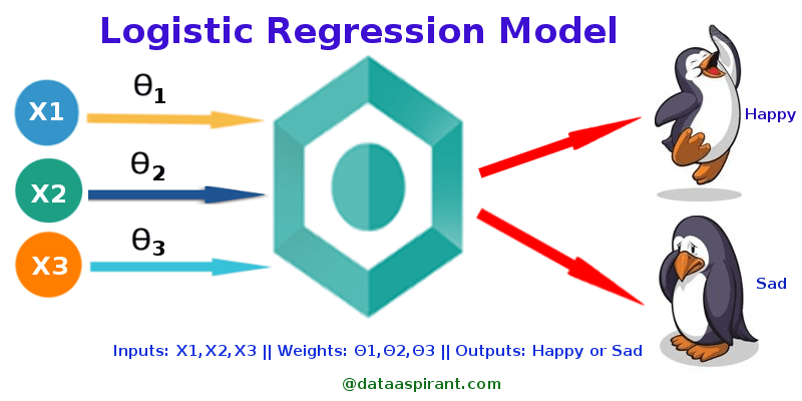
\includegraphics[scale=0.3]{4.png}
	\caption{Logistic regression is a classic machine learning algorithom used for calssification task. As shown in the picture, we first feed the data, the inputs to the model, and the model gives us its classification result.
	}
\end{figure}

\end{frame}
%------------------------------------------------
%\subsection{Definition}
\begin{frame}
\frametitle{Introduction}
\begin{block}{Basic idea:}
	\begin{itemize}
		\item $f(Z)=h_{\theta}(x)=sigmoid(Z)=\frac{1}{1+e^{-Z}}$
		\item Output = 0 or 1
		\item $Hypothesis \longrightarrow Z=W_x+B$
	\end{itemize}
\end{block}
We usually attach the sigmod function to the end of the model, it gives us the probaility of the label being 1
\begin{figure}[h]
	\centering
	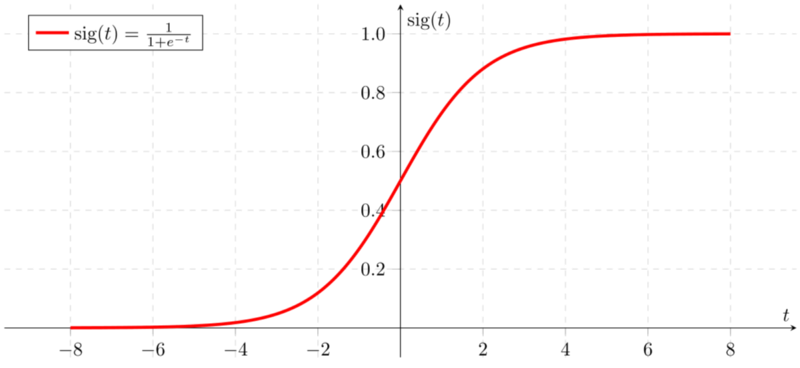
\includegraphics[scale=0.3]{5.png}
	\caption{If ��Z�� goes to infinity, Y(predicted) will become 1 and if ��Z�� goes to negative infinity, Y(predicted) will become 0.	
	}
\end{figure}
\end{frame}

\subsection{Loss Function}
\begin{frame}
	\frametitle{Loss Function}
	Predicted Probability:
	$$
	P(y=1|x)=h\theta(x)=\frac1{1+e^(-\theta^Tx)}=\delta(\theta^Tx)\eqno{(3)}
	$$
	$$
	P(y=0|x)=1-P(y=1|x)=1-h_\theta(x)\eqno{(4)}
	$$
	Combined (3).(4):
	$$
	P(y|x;0)=(h_\theta(x))^y(1-h_\theta(x))^{1-y^{\color{red}\text{y stands for the labels, being 0 or 1}}}\eqno{(5)}
	$$
	
	Using maximum likelihood estimation(MLE) according to the m given samples:
	$$
	L(\theta)=\prod^m_{i=1}P(y^{(i)}|x^{(i)};\theta)=\prod^m_{i=1}(h_\theta(x^{(i)}))y^{(i)}(1-h_\theta(x^{(i)}))^{1-y^{(i)}} \eqno{(6)}
	$$
	$$
	\longrightarrow l(\theta)=\log L(\theta)=\sum^m_{i=1}(y^{(i)}\log h_\theta(x^{(i)})+(1-y^{(i)})\log (1-h_\theta(y^{(i)})))\eqno{(7)}
	$$
	
	$$
	J(\theta)=-\frac{1}{m}l(\theta)\eqno{\color{red}\text{$J(\theta)$ is the desired loss function
	}}
	$$
	
\end{frame}
%%------------------------------------------------
\subsection{Regularization}
\begin{frame}
\frametitle{Regularization}
\begin{block}{Basic idea}
	\begin{itemize}
		\item L2$$
		J(\theta)=\frac{1}{2m}[\sum^m_{i=1}(h_\theta(x^{(i)}))^2+\lambda\sum^n_{j=1}\theta^2_j] \eqno{(8)}
		$$
		\item Regularization : prevent the weights from getting too large
		\item Regularization can avoid overfitting to some extent through the restraint of weights
	\end{itemize}
\end{block}
\end{frame}

\begin{frame}
\frametitle{Regularization}
\begin{figure}[h]
	\centering
	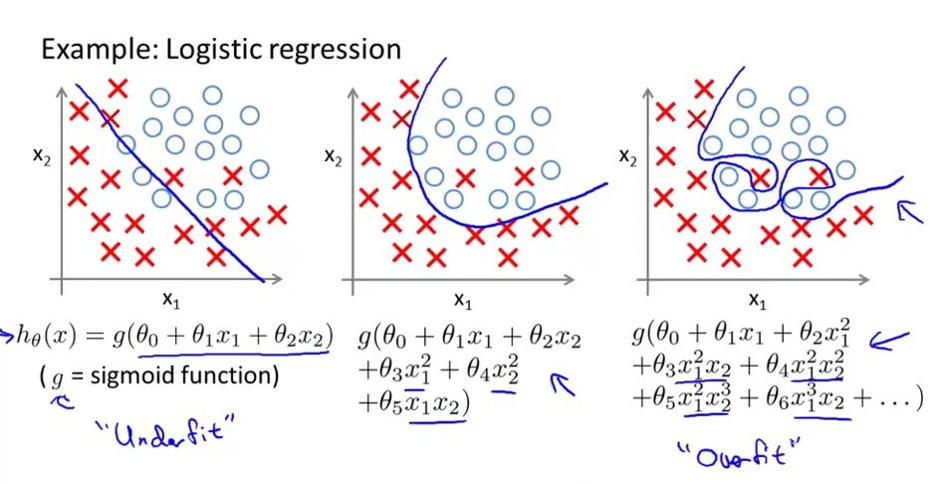
\includegraphics[scale=0.4]{6.png}
	\caption{Underfitting/overfitting
	}
\end{figure}
\end{frame}


\begin{frame}
\frametitle{Regularization}
Classification task through Logistic Regression
\begin{figure}[h]
	\centering
	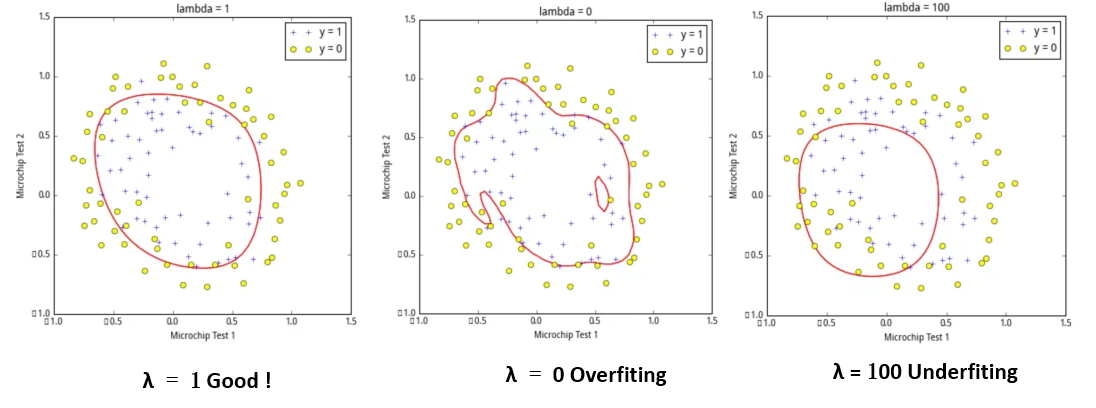
\includegraphics[scale=0.3]{7.png}
	\caption{Two-class classification when �� has different values
	}
\end{figure}
\end{frame}


\subsection{Weights Learning of LR}
\begin{frame}
\frametitle{Gradient Descent}
\begin{figure}[h]
	\centering
	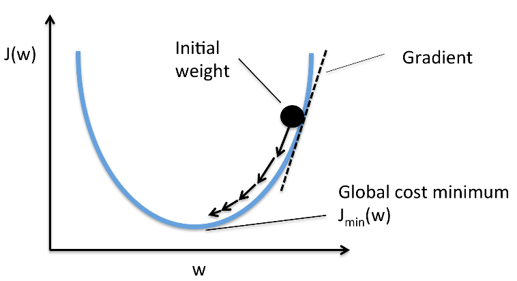
\includegraphics[scale=0.7]{8.png}
\end{figure}
\begin{figure}[h]
	\centering
	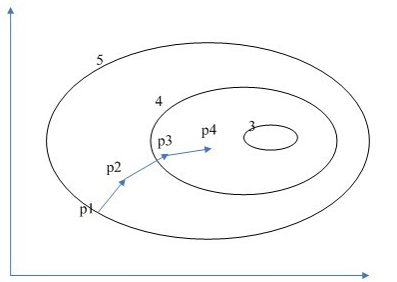
\includegraphics[scale=0.7]{9.png}
\end{figure}
\end{frame}
\begin{frame}
\frametitle{Gradient Descent}
$$
J(\theta)=-\sum^m_{i=1}(y^{(i)}\log h_\theta(x^{(i)})+(1-y^{(i)})\log (1-h_\theta(y^{(i)})))\eqno{(9)}
$$
$$\downarrow$$
Partial derivative:
$$\frac{\partial J(\theta)}{\partial \theta_j}=\sum_ix_j^{(i)}(h_\theta(x^{(i)})-y^{(i)})$$
$$\downarrow$$
Weights update:
$$\theta_j=\theta_j-\alpha\frac{\partial J(\theta)}{\partial J(\theta_j)}$$
\end{frame}

\section{Logistic Regression vs Naive Bayes}
\subsection{Comparison}
\begin{frame}
	\frametitle{Comparison}
	\begin{block}{Basic idea}
		\begin{itemize}
			\item Machine learning algorithms can be (roughly) categorized into two categories:
			\item Generative algorithms, that estimate $P(x_i,y)$ (often they model $P(x_i|y)$ and $P(y)$ separately).
			\item Discriminative algorithms, that model $P(y|x_i)$
		\end{itemize}
	\end{block}
1. The Naive Bayes algorithm is generative. ($p(y),p(x|y) \rightarrow p(y|x)$)
$$
P(y|x)=\frac{p(x,y)}{\prod_yp(x,y)}=\frac{p(y)p(x|y)}{\prod_yp(y)p(x|y)}
$$

2. Logistic Regression is discriminative. (Gradient descent$\rightarrow w$)
$$
P(y|x_i)=\frac1{1+e^{y(w^Tx_i+b)}}
$$
\end{frame}
%%------------------------------------------------
%\section{Reference}
%------------------------------------------------
%\begin{frame}
%\frametitle{Reference}
%\begin{thebibliography}{4}
%\bibitem{LS-SPH} F. Zou, C. Liu, H. Ling, H. Feng, L. Yan, and D. Li, "Least square regularized spectral hashing for similarity search," Signal Processing, vol. 93, pp. 2265-2273, 2013. (SCI,EI)
%\bibitem{KMFH} F. Zou, Y. Chen, J. Song, K. Zhou, Y. Yang, and N. Sebe, "Compact image fingerprint via multiple kernel hashing," IEEE Transactions on Multimedia, vol. 17, pp. 1006-1018, 2015. (SCI,EI)
%\bibitem{KNPH} C. Liu, H. Ling, F. Zou, L. Yan, Y. Wang, H. Feng, et al., "Kernelized neighborhood preserving hashing for social-network-oriented digital fingerprints," IEEE Transactions on Information Forensics and Security, vol. 9, pp. 2232-2247, 2014. (SCI,EI)
%\bibitem{DTSH} Liu, Yu; Song, Jingkuan; Zhou, Ke; Yan, Lingyu; Liu, Li; Zou, Fuhao; Shao, Ling, "Deep Self-taught Hashing for Image Retrieval," IEEE Tra
%\bibitem{DeepFace} Fuhao Zou, Fan Yang, Wei Chen,Kai Lia, Jingkuan Song, Jingcai Chen, Hefei Ling, "Fast Large Scale Deep Face Search," Pattern Recognition Letters, Januray 3, 2019. (SCI,EI)
%\end{thebibliography}
%\end{frame}
%------------------------------------------------
\begin{frame}
\Huge{\centerline{The End}}
\end{frame}
\end{CJK*}
\end{document}
%\end{document}
